\documentclass[runningheads,a4paper]{llncs}

\usepackage[draft]{fixme}
%\usepackage{times}
\usepackage{url}
\usepackage{latexsym}

\usepackage{amsmath, amssymb, xspace, enumerate}

\usepackage{tikz}
\usetikzlibrary{automata}

\usepackage[ruled,vlined]{algorithm2e}
%%% Opciones de algorithms2e (para que ocupen menos)
  % margen chiquito
\setlength{\algomargin}{9pt}
  % no usar punto-y-coma
%\DontPrintSemicolon
\renewcommand{\algorithmcfname}{\small Algorithm}

\usepackage{mathtools}

\usepackage{relsize}

\usepackage{hyperref}

% para que los align puedan cortarse
\allowdisplaybreaks

% esto controla la separaci�n de los floats respecto al texto. necesitamos el espacio extra!
\addtolength{\textfloatsep}{-13pt}
\addtolength{\intextsep}{-8pt}

% Compiling version
\newif\iffullversion\fullversionfalse

% for compatibility with older versions of algorithm2e
\providecommand{\LinesNumbered}{\linesnumbered}
\providecommand{\dontprintsemicolon}{\DontPrintSemicolon}

\newcommand{\pr}[2]{{\it pre}_{#1}(#2)}
\newcommand{\su}[2]{{\it suc}_{#1}(#2)}
\newcommand{\guard}{$\exists r,u,v,w:v \in
\su{r}{u},w\in S(u),\su{r}{w}\cap S(v)=\emptyset$}
\newcommand{\unary}{P}



\newcommand{\findcite}{\cite{XXX}\fixme{cite!}\xspace}

\newcommand{\FOL}{\ensuremath{\mathcal{FO}}\xspace}
\newcommand{\EPFOL}{\ensuremath{{\FOL^-}}\xspace}
\newcommand{\ALC}{\ensuremath{\mathcal{ALC}}\xspace}
\newcommand{\EL}{\ensuremath{\mathcal{EL}}\xspace}
\newcommand{\ELAN}{\ensuremath{{\mathcal{EL}^+}}\xspace}

\newcommand{\st}{\mathit{\tau}\xspace}

\newcommand\+[1]{\mathcal{#1}}

\newcommand{\simil}[1]{\mathrel{\stackrel{\mathsmaller{#1}}{\raisebox{-.07em}{$\rightsquigarrow$}}}}
\newcommand{\simul}[1]{\mathrel{\stackrel{\mathsmaller{#1}}{\underline{\makebox[.75em][l]{\hspace{-.05em}\raisebox{-.15ex}{$\rightarrow$}}}}}}

\newcommand{\ext}[1]{\|#1\|}
\newcommand{\size}[1]{\# #1}
\newcommand{\leqs}{\leq_s}

\newcommand{\atomL}{\textsc{atom}_L\xspace}
\newcommand{\atomR}{\textsc{atom}_R\xspace}
\newcommand{\atomLR}{\textsc{atom}_{L/R}\xspace}

\newcommand{\zig}{\textsc{rel}_L\xspace}
\newcommand{\zag}{\textsc{rel}_R\xspace}
\newcommand{\zigzag}{\textsc{rel}_{L/R}\xspace}

\newcommand{\injL}{\textsc{inj}_L\space}
\newcommand{\injR}{\textsc{inj}_R\space}
\newcommand{\injLR}{\textsc{inj}_{L/R}\space}

\newcommand{\diam}{\exists r.}
\newcommand{\NN}{\mathbb{N}}
\newcommand{\QQ}{\mathbb{Q}}
\newcommand{\RR}{\mathbb{R}}

\newcommand{\pos}{\EL}
\newcommand{\posre}{$\pos$-RE\xspace}
\newcommand{\Id}{{\rm Id}}
\renewcommand{\phi}{\varphi}
\newcommand{\simmax}{\sim^m}
\newcommand{\dom}{{\rm dom}}
\newcommand{\remove}{{\it remove}}
\newcommand{\prevS}{{\it prevS}}
\newcommand{\form}{{\it form}}
\newcommand{\simset}{{\it sim}}
\newcommand{\pred}{{\it pre}}
\newcommand{\post}{{\it post}}

\newcommand{\io}{
\SetKwInOut{Input}{input}\SetKwInOut{Output}{output}
\Input{a finite model $\gM=\tup{\Delta,\interp{\cdot}}$}
\Output{$\forall v\in \Delta$, a formula $F(v) \in \EL$, and  the
simulator set $S(v)$ such that $\interp{F(v)}=S(v)=\simset_\EL(v)$}
\BlankLine}

\newcommand{\pair}[2]{\langle #1,#2\rangle}
\newcommand{\rg}{{\rm rg}}

\newcommand{\tup}[1]{\langle #1\rangle}
\newcommand{\cset}[1]{\{#1\}}

\newcommand{\gM}{\mathcal{M}}
\newcommand{\gG}{\mathcal{G}}
\newcommand{\gL}{\mathcal{L}}
\newcommand{\interp}[1]{|\!|#1|\!|}
\newcommand{\rel}{\ensuremath{\mathsf{rel}}\xspace}
\newcommand{\prop}{\ensuremath{\mathsf{prop}}\xspace}

\newcommand{\sect}[1]{\S\ref{sec:#1}}

%\theoremstyle{plain}
%\newtheorem{thm}{Theorem}
%\newtheorem{propos}[thm]{Proposition}
%\newtheorem{lem}[thm]{Lemma}
%\newtheorem{cor}[thm]{Corollary}
%\newtheorem{fact}[thm]{Fact}
%\newtheorem{defn}[thm]{Definition}
%\theoremstyle{remark}
%\newtheorem{ex}[thm]{Example}

%\pagestyle{plain}  % switches on printing of running heads

\spnewtheorem{convention}{Convention}{\bfseries}{}

\iffullversion
\title{Referring Expressions modulo Expressiveness\\{\sc(full version)}}
\else
\title{Using Logic in the
Generation of Referring Expressions}
\fi
%
\author{%
Carlos Areces\inst{1}
\and%
Santiago Figueira\thanks{S.~Figueira was partially
supported by CONICET (grant PIP 370) and UBA (grant UBACyT 20020090200116).}\inst{2}
\and%
Daniel Gor\'in\inst{3}
}


\institute{INRIA Nancy, Grand Est, France\\
\email{areces@loria.fr}\\
\and
Departamento de Computaci\'on, FCEyN, UBA and CONICET,
Argentina
\and
Departamento de Computaci\'on, FCEyN, UBA, Argentina\\
\email{\{santiago,dgorin\}@dc.uba.fr}}

\date{}

\begin{document}
\maketitle
\begin{abstract}
The problem of generating referring
expressions (GRE) is an important task in natural language generation.
In this paper, we advocate for the use of logical languages in
the output of the content determination phase (i.e., when the
relevant features of the object to be referred are selected).
Many different logics can be used for this and we argue that, for a
particular application, the actual choice shall 
constitute a compromise between expressive power (how many objects
can be distinguished), computational complexity (how difficult
it is to determine the content) and realizability (how often will the
selected content be realized to an idiomatic expression). We show that
well-known results from the area of computational logic can then be transferred
to GRE. Moreover, our approach is orthogonal
to previous proposals and we illustrate this by generalizing well-known 
content-determination algorithms to make them parametric on the
logic employed.

%We provide new complexity
%bounds, discuss the issue of the length of the generated
%descriptions, and propose ways in which the two approaches discussed
%in this article can be combined.
\end{abstract}


\subsection{Descripci\'on del problema}


En linguistica una expresi\'on referencial (RE) es una expresi\'on que identifica un\'{ì}vocamente a un objeto de para un interlocutor, 
desde un conjunto de posibles distractores. Por ejemplo si nosotros queremos identificar a un cierto animal d de un conjunto de mascotas, 
la expresi\'on ``el perr'' ser\'a ER si d es el \'unico perro en el conjunto, y si nosotros estamos seguros que nuestro interlocutor 
identificar\'a a d como un perro.


\subsection{Contribuciones}

\begin{itemize}
 \item Un algoritmo para la generaci\'on de expresiones referenciales independiente de dominio.
 \item
\end{itemize}

\subsection{Mapa de la tesis}
Esta tesis se divide en 6 cap\'{i}tulos, en el primer cap\'{i}lo ...


\newcommand{\nDog}{\mathit{dog}\xspace}
\newcommand{\nCat}{\mathit{cat}\xspace}
\newcommand{\aSmall}{\mathit{small}\xspace}
\newcommand{\aSniffing}{\mathit{sniffs}\xspace}
\newcommand{\nBreed}{\mathit{beagle}\xspace}


\section{Measuring Expressive Power}\label{sec:technical}

Relational structures are very suitable for representing \emph{situations} or
\emph{scenes}.  A relational structure (also called ``relational model'') is a non-empty
set of objects --the \emph{domain}-- together with a collection of relations, each with a fixed arity.

Formally, assume a fixed and finite (but otherwise arbitrary)
vocabulary of $n$-ary relation symbols.\footnote{
  Constants and function symbols can be represented as relations of
  adequate arity.}
A relational model $\+M$ is a tuple
$\tup{\Delta,\interp{\cdot}}$ where $\Delta$ is a nonempty set, and
$\interp{\cdot}$ is a suitable interpretation function, that is,
$\interp{r} \subseteq \Delta^n$ for every $n$-ary relation symbol
$r$ in the vocabulary. We say that $\+M$ is \emph{finite} whenever
$\Delta$ is finite.  The \emph{size} of a model $\+M$ is the sum
$\#\Delta + \#\interp{\cdot}$, where $\#\Delta$ is the cardinality
of $\Delta$ and $\#\interp{\cdot}$ is the sum of the sizes of all
relations in $\interp{\cdot}$.

Figure~\ref{fig:cat-dog-1} below shows how we can represent a scene
as a relational model. Intuitively, $a$, $b$ and $d$ are dogs, while
$c$ and $e$ are cats;  $d$ is a small beagle;
 $b$ and $c$ are also small.
 We read $\aSniffing(d,e)$ as ``{\em $d$ is sniffing $e$}''.

 \begin{figure}
 \begin{center}
 \begin{tabular}{rcl}
$\Delta$               & = & $\cset{a,b,c,d,e}$\\
$\interp{\nDog}$      & = & $\cset{a,b,d}$\\
$\interp{\nCat}$      & = & $\cset{c,e}$\\
$\interp{\nBreed}$    & = & $\cset{d}$\\
$\interp{\aSmall}$    & = & $\cset{b,c,d}$\\
$\interp{\aSniffing}$ & = & $\cset{(a,a),(b,a),(c,b),(d,e),(e,d)}$
 \end{tabular}
\begin{picture}(120,50)
\put(0,-50){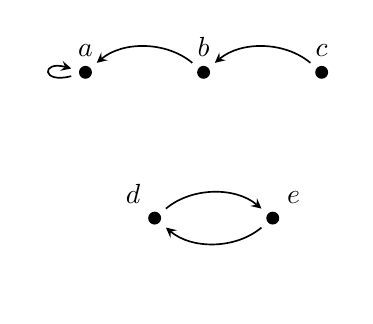
\begin{tikzpicture}
  [
    n/.style={circle,fill,draw,inner sep=1.5pt,node distance=1.5cm},
    aSniffing/.style={->, >=stealth, semithick, shorten <= 3pt, shorten >= 3pt},
  ]
 \node[n,label=above:$a$,label=below:{\relsize{-1}$\begin{array}{c}\nDog\end{array}$}] (a) {};

 \node[n,label=above:$b$,label=below:{\relsize{-1}$\begin{array}{c}\nDog\\ \aSmall \end{array}$}, right of=a] (b) {};

 \node[n,label=above:$c$,label=below:{\relsize{-1}$\begin{array}{c}\nCat\\ \aSmall\end{array}$}, right of=b] (c) {};

 \node[n,label=above left:$d$,label=below:{\relsize{-1}$\begin{array}{c}\nDog\\ \nBreed\\  \aSmall \end{array}$}, below of=a,xshift=25pt,yshift=-10pt] (d) {};

 \node[n,label=above right:$e$,,label=below:{\relsize{-1}$\begin{array}{c}\nCat\end{array}$},right of=d] (e) {};

 \draw [aSniffing,loop left] (a) to node[above,xshift=-5pt]{\relsize{-1}$\aSniffing$} (a);

 \draw [aSniffing,bend right=40] (b) to node[auto,swap]{\relsize{-1}$\aSniffing$} (a);

 \draw [aSniffing,bend right=40] (c) to node[auto,swap]{\relsize{-1}$\aSniffing$} (b);

 \draw[aSniffing, bend left=40] (d) to node[auto]{\relsize{-1}$\aSniffing$} (e);
 \draw[aSniffing, bend left=40] (e) to node[auto,swap]{\relsize{-1}$\aSniffing$} (d);

 \end{tikzpicture}}
 \end{picture}

 \end{center}
 \caption{Graph representation of scene $\+S$.\label{fig:cat-dog-1}}
 \end{figure}


Logical languages are fit for the task  of (formally) \emph{describing}
elements of a relational structure. Consider, e.g., the classical language
of first-order logic (with equality), \FOL, given by:
$$
  \top \mid x_i \not\approx x_j \mid  r (\bar x) \mid \lnot \gamma \mid \gamma \land \gamma' \mid \exists x_i . \gamma
$$
%
where $\gamma,\gamma' \in \FOL$,
$r$ is an $n$-ary relation symbol and $\bar x$ is an $n$-tuple of variables.
As usual, $\gamma \lor \gamma'$ and $\forall x . \gamma$ are short for
$\lnot(\lnot\gamma \land \lnot\gamma')$ and $\lnot\exists x . \lnot\gamma$, respectively.
Formulas of the form $\top$, $x_i \not\approx x_j$ and $r(\bar
x)$ are called \emph{atoms}.%
  \footnote{%
    For technical reasons, we include the inequality symbol $\not \approx$ as
    primitive.  Equality can be defined using negation.
  }
Given a relational model $\+M = \tup{\Delta,\interp{\cdot}}$ and a
formula $\gamma$ with free variables%
\footnote{%
    W.l.o.g.\ we assume that no variable appears both free and bound, that no variable is bound
    twice, and that the index of bound variables in a formula increases from left to right.%
}
among $x_1\ldots x_n$, we inductively define the \emph{extension} or
\emph{interpretation} of  $\gamma$ as the set of $n$-tuples
 $\interp{\gamma}^n \subseteq \Delta^n$ that satisfy:

\begin{center}
\begin{tabular}{rcl@{\hspace{1cm}}rcl}
$\interp{\top}^n$ &$=$& $\Delta^n$
&
$\interp{x_i \not\approx x_j}^n$ &$=$& $\cset{\bar{a} \mid \bar{a} \,{\in}\, \Delta^n, a_i \neq a_j}$
\\
$\interp{\lnot\delta}^n$ &$=$& $\Delta^n \setminus \interp{\delta}^n$
&
$\interp{r (x_{i_1} \ldots x_{i_k})}^n$ & $=$&$\cset{\bar{a} \mid \bar{a} \,{\in}\, \Delta^n, (a_{i_1} \ldots a_{i_k}) {\in} \interp{r}}$
\\
$\interp{\delta \land \theta}^n$ &$=$& $\interp{\delta}^n \cap \interp{\theta}^n$
&
$\interp{\exists x_{l}.\delta}^n$ &$=$& $\cset{\bar a \mid \bar a  e  \in \interp{\delta'}^{n+1}\ \text{for some $e$}}$
\end{tabular}
\end{center}
%
where $1 \le i,j, i_1, \ldots, i_k \le n$, $\bar{a} = (a_1\ldots
a_n)$, $\bar{a}e = (a_1\ldots a_n,e)$ and $\delta'$ is
obtained by replacing all occurrences of $x_l$ in $\delta$ by
$x_{n+1}$. When the cardinality of the tuples involved is known from
the context we will just write $\interp{\gamma}$ instead of
$\interp{\gamma}^n$.

With a language syntax and semantics in place, we can now formally
define the problem of $\+L$-GRE for a target set of elements $T$
(we slightly adapt the definition in~\cite{AKS08}):

\medskip
\noindent
{\small
\begin{center}
\begin{tabular}{ll} \hline
\multicolumn{2}{l}{
\textsc{$\gL$-GRE Problem}}\\ \hline
\ \ Input: & a model $\gM=\tup{\Delta,\interp{\cdot}}$ and a nonempty target  set $T \subseteq \Delta$.\\
\ \ Output: & a formula $\varphi \in \gL$ such that
$\interp{\varphi} = T$ if it exists, and $\bot$ otherwise.\\ \hline
\end{tabular}
\end{center}}
When the output is not $\bot$, we say that $\phi$ is an
\emph{$\+L$-referring expression ($\+L$-RE) for $T$ in $\+M$}.
Simply put then, the output of the $\+L$-GRE problem is a formula of
$\+L$ whose interpretation in the input model is the target set, if
such a formula exists.  This definition applies also to the GRE for
objects of the domain by taking a singleton set as target.

By using  formulas with $n$ free variables one could extend
this definition to describe $n$-ary relations; but here we are only
interested in describing  subsets of the domain. Actually, we shall
restrict our attention a little further:

\begin{convention}\label{conv:signature}
We will only consider relational models with unary and binary relation
symbols (i.e., labeled graphs).  We will consistently use $p$ for a unary relation
symbol (and called it a \emph{proposition}) and $r$ for a binary relation symbol.
\end{convention}

\noindent
This convention captures the usual models of interest when describing scenes
as the one presented in Figure~\ref{fig:cat-dog-1}.  Accommodating relations of
higher arity in our theoretical framework is easy, but it might affect computational complexity.

\subsection{Choosing the Appropriate Language}\label{sec:choosinglanguage}

Given a model $\+M$, there might be an infinite number of formulas
that uniquely describe a target (even formulas which are not
logically equivalent might have the same interpretation once a model
is fixed). Despite having the same interpretation in $\+M$, they may
be quite different with respect to other parameters.

As it is well known in the automated text
generation community, different realizations of the same content
might result in expressions which are more or less appropriate in a given context. Although,
as we mentioned in the introduction, we will only address the
content determination part (and not the surface realization part)
of the GRE problem, we will argue that generating content using languages with
different expressive power can have an impact in the
posterior surface generation step.

Let us consider again the scene in Figure~\ref{fig:cat-dog-1}.
Formulas $\gamma_1$--$\gamma_4$ shown in Table~\ref{tab:gammas}
are all such that $\gamma_i$ uniquely describes $b$
(i.e., $\interp{\gamma_i} = \cset{b}$) in model $\+S$.
Arguably, $\gamma_1$ can be easily realized as \emph{``the small dog
that sniffs a dog''}. Syntactically, $\gamma_1$ is characterized as
a positive, conjunctive, existential formula (i.e., it contains no
negation and uses only conjunction and existential quantification).
Expressions with these characteristics are, by large, the most
commonly found in corpora as those compiled
in~\cite{viet:algo06,deem:buil06,dale:refe09}. Formula $\gamma_2$, on the
other hand, contains negation, disjunction and universal
quantification. It could be realized as \emph{``the small dog that
only sniffs things that are not cats''} which sounds unnatural. Even
a small change in the form of $\gamma_2$ makes it more palatable:
rewrite it using $\exists$, $\lnot$, and $\land$ to obtain
\emph{``the small dog that is not sniffing a cat''}. Similarly,
 $\gamma_3$ and $\gamma_4$ seem computationally harder to
realize than $\gamma_1$: $\gamma_3$ contains an inequality
(\emph{``the dog sniffing another dog''}), while the quantified
object appears in the first argument position in the binary relation
in $\gamma_4$ (\emph{``the dog that is sniffed by a small cat''}).

Summing up, we can ensure, already during the content determination
phase, certain properties of the generated referring expression by
paying attention to the formal language used in the representation.
And we can do this, even before taking into account other
fundamental linguistics aspects that will make certain realization
preferable like saliency, the cognitive capacity of the hearer (can
she recognize a \emph{beagle} from another kind of dog?), etc.

%
\begin{table}
$$
\begin{array}{cl}
 \gamma_1: & \nDog(x) \land \aSmall(x) \land
   \exists y . (\aSniffing(x,y) \land \nDog(y))\\[3pt]
  %
  \gamma_2: & \nDog(x) \land \aSmall(x) \land
  \forall y . (\neg \nCat(y) \lor \neg \aSniffing(x,y))\\[3pt]
  %
  \gamma_3: & \nDog(x) \land
  \exists y . (x \not\approx y \land \nDog(y)  \land \aSniffing(x,y))\\[3pt]
  %
  \gamma_4: & \nDog(x) \land
  \exists y . (\nCat(y) \land \aSmall(y) \land \aSniffing(y,x))
  %
 \end{array}
$$
\caption{Alternative descriptions for object $b$ in the model shown in Figure~\ref{fig:cat-dog-1}.}\label{tab:gammas}
\end{table}
%


%the content determination problem can be seen as that of generating a certain logical
%formula, but not just any formula. It is not simple to characterize which formulas are not acceptable
%but one can approximate it by restricting to formulas of certain shape.

As a concrete example, let \EPFOL be the fragment of \FOL-formulas where the operator $\lnot$
does not occur (but notice that atoms $x_i \not\approx x_j$ are permitted).
By restricting content determination to \EPFOL, we ensure that formulas like  $\gamma_2$
will not be generated.
If we  ban $\not\approx$ from the language, $\gamma_3$ is precluded.

The fact that the representation language used has an impact on content
determination is obvious, but it has not received the attention it deserves.
Areces~et~al.~\cite{AKS08} use different description logics (a family of formal languages
used in knowledge representation, see~\cite{baad:desc03}) to classify, and
give a formal framework to previous work on GRE.  Let us quickly introduce
some of these languages as we will be mentioning them in future sections.  Using
description logics instead of \FOL fragments is just a notational issue, as most
description logics can be seen as implicit fragments of \FOL.
For example, the language of the description logic \ALC, syntactically defined
as the set of formulas,
$$
\top \mid p \mid \neg \gamma \mid \gamma \wedge \gamma' \mid  \exists r. \gamma
$$
(where $p$ is a propositional symbol, $r$ a binary relational symbol, and $\gamma,\gamma' \in \ALC$) corresponds to a syntactic fragment of
\FOL without $\not\approx$, as shown by the standard translation  $\st_x$:

\begin{center}
\begin{tabular}{rcl@{\hspace{1cm}}rcl}
$ \st_{x_i}(\top)$ &$=$& $\top$
&
$\st_{x_i}(\gamma_1 \land \gamma_2)$ &$=$& $\st_{x_i}(\gamma_1) \land \st_{x_i}(\gamma_2)$
\\
  $\st_{x_i}(p)$ &$=$& $p(x_i)$
&
$\st_{x_i}(\exists r . \gamma)$ &$=$& $\exists x_{i+1} . (r(x_i,x_{i+1}) \land \st_{x_{i+1}}(\gamma))$
\\
 $\st_{x_i}(\lnot \gamma)$ &$=$& $\lnot\st_{x_i}(\gamma)$
&
\end{tabular}
\end{center}
%
% \begin{align*}
%  \st_{x_i}(\top) &= \top
% \\
%   \st_{x_i}(p) &= p(x_i)
% \\
%  \st_{x_i}(\lnot \gamma) &= \lnot\st_{x_i}(\gamma)
% \\
%  \st_{x_i}(\gamma_1 \land \gamma_2) &= \st_{x_i}(\gamma_1) \land \st_{x_i}(\gamma_2)
% \\
%  \st_{x_i}(\exists r . \gamma) &= \exists x_{i+1} . (r(x_i,x_{i+1}) \land \st_{x_{i+1}}(\gamma))
% \end{align*}

Indeed, given a relational model $\+M$, the extension of an \ALC formula $\varphi$ in $\+M$ exactly coincides
with the extension of $\st_{x_1}(\varphi)$ (see, e.g.,~\cite{baad:desc03}).  Thanks
to this result, for any formula $\varphi$ of \ALC and its sublanguages we can
define $\interp{\varphi} = \interp{\st_{x_1}(\varphi)}$.  Coming back to our previous example,
 by restricting content generation to $\ALC$ formulas (or equivalently, the corresponding
 fragment of \FOL) we would avoid
formulas like $\gamma_3$ (no equality) and $\gamma_4$ (quantified
element appears always in second argument position).

Generation is discussed in~\cite{AKS08} in terms of different description
logics like \ALC and \EL (\ALC without negation). We will  extend the results
in that paper, considering for instance \ELAN (\ALC with negation allowed only
in front of unary relations) but, more generally, we take a model theoretic
approach and argue that the primary question is not whether one should use one
or other (description) logic for content generation, but rather which are the
\emph{semantic differences} one cares about. This determines the
required logical formalism but also impacts on both the
content determination and the surface realization problems.
Each logical language can be seen as a compromise between expressiveness,
realizability and computational complexity. The appropriate selection for a particular
GRE task should depend on the actual context.
%As we will see, the
%move from one logical language to another impacts not only on the
%shape of formulas that can be generated but also on the
%computational complexity of the generation problem, and on its
%success, i.e., when it will be possible to uniquely identify a given
%target.

\subsection{Defining \emph{Sameness}}

Intuitively,  given a logical language $\+L$ we say that an object $u$ in a model
$\+M_1$ is similar in $\+L$ to
an object $v$ in a model $\+M_2$ whenever all $\+L$-formulas satisfied by $u$ are also
satisfied by $v$. Formally,
%let $\+L$ stand for any of the languages discussed so far, and
let $\+M_1 = \tup{\Delta_1, \interp{\cdot}_1}$ and $\+M_2 = \tup{\Delta_2, \interp{\cdot}_2}$ be
two relational models with $u \in \Delta_1$ and $v \in \Delta_2$;
we follow the terminology of~\cite{AKS08} and say that
\emph{$u$ is $\+L$-similar to $v$}  (notation $u \simil{\+L} v$) whenever $u \in \interp{\gamma}_1$ implies
$v \in \interp{\gamma}_2$, for every $\gamma \in \+L$. It is easy to show that
$\+L$-similarity is reflexive for all $\+L$, and symmetric  for languages that contain negation.

Observe that $\+L$-similarity captures the notion of
`identifiability in $\+L$'. If we take $\+M_1$ and $\+M_2$ to be the
same model, then an object $u$ in the model can be uniquely
identified using $\+L$ if there is no object $v$ different from $u$
such that $u \simil{\+L} v$. In other words, if there are two
objects $u$ and $v$  in a model $\+M$ such that $u \simil{\+L} v$,
then the $\+L$-GRE problem with input $\+M$ and target $T=\{u\}$
will not succeed since for all formulas $\gamma \in L$ we have
$\{u,v\} \subseteq \interp{\gamma} \not = \{u\}$.

The notion of $\+L$-similarity then, gives us a handle on the
$\+L$-GRE problem. Moreover, we can recast this definition in a
structural way, so that we do not need to consider infinitely many
$\+L$-formulas to decide whether $u$ is $\+L$-similar to $v$.  We
can reinterpret $\+L$-similarity in terms of standard
model-theoretic notions like isomorphisms or bisimulations which
describe structural properties of the model, instead. Given two
models $\tup{\Delta_1, \interp{\cdot}_1}$ and $\tup{\Delta_2,
\interp{\cdot}_2}$, consider the following properties of a binary
relation ${\sim} \subseteq \Delta_1 \times \Delta_2$ (cf.~Convention~\ref{conv:signature}):
\smallskip


%\begin{description}
%\item[\smaller$\atomL$:] If $u_1{\sim} u_2$, then $u_1 \in \interp{p}_1 \Rightarrow u_2 \in \interp{p}_2$.
%\item[\smaller$\atomR$:] If $u_1{\sim} u_2$, then $u_2 \in \interp{p}_2 \Rightarrow u_1 \in \interp{p}_1$.
%\item[\smaller$\zig$:] If $u_1{\sim} u_2$ and $(u_1,v_1) \in \interp{p}_1$, then $v_1{\sim}v_2$
%  and $(u_2,v_2) \in \interp{p}_2$, for some $v_2$.
%\item[\smaller$\zag$:] If $u_1{\sim}u_2$ and $(u_2,v_2) \in \interp{p}_2$, then $u_1{\sim}v_1$ and
% $(u_1,v_1) \in \interp{p}_1$, for some $v_1$.
%\item[\smaller$\injL$:] $\sim$ is an injective function $\Delta_1 \to \Delta_2$.
%\item[\small$\injR$:] $\sim^{-1}$ is an injective function $\Delta_2 \to \Delta_2$.
%\end{description}

\newcommand{\simdef}[2]{\noindent\ \ #1\hfill:\ \parbox[t]{.87\textwidth}{#2}\par}

\simdef{$\atomL$}{If $u_1{\sim} u_2$, then $u_1 \in \interp{p}_1 \Rightarrow u_2 \in \interp{p}_2$}
\simdef{$\atomR$}{If $u_1{\sim} u_2$, then $u_2 \in \interp{p}_2 \Rightarrow u_1 \in \interp{p}_1$}
\simdef{$\zig$}{If $u_1{\sim} u_2$ and $(u_1,v_1) \in \interp{r}_1$, then $\exists v_2$ s.t.\ $v_1{\sim}v_2$
  and $(u_2,v_2) \in \interp{r}_2$}
\simdef{$\zag$}{If $u_1{\sim}u_2$ and $(u_2,v_2) \in \interp{r}_2$, then $\exists v_1$ s.t.\ $u_1{\sim}v_1$ and
 $(u_1,v_1) \in \interp{r}_1$}
\simdef{$\injL$}{$\sim$ is an injective function (when restricted to its domain)}
\simdef{$\injR$}{$\sim^{-1}$ is an injective function (when restricted to its domain)}
\smallskip

We will say that a non-empty binary relation $\sim$ is an
\emph{$\+L$-simulation} when it satisfies the properties indicated
in Table~\ref{tab:simuls}. For example, a non-empty binary relation that satisfies $\atomL$, and $\zig$ is an $\EL$-simulation, as indicated in row~4 of Table~\ref{tab:simuls}. Moreover, we will say that an object
\emph{$v$ $\+L$-simulates $u$} (notation $u \simul{\+L} v$) if there
is a relation $\sim$ satisfying the corresponding properties such that
$u \sim v$. The following is a fundamental model-theoretic result:%~\cite{ebbi:math96,KR99,BRV01}

\begin{table}[t]
$$
\begin{array}{c|cccccc}
  \+L & \atomL & \atomR & \zig & \zag & \injL & \injR \\
  \hline
  \FOL   & \times & \times & \times & \times & \times & \times\\
  \EPFOL & \times & & \times && \times &\\
  \ALC   & \times & \times & \times & \times&&\\
  \EL    & \times & &  \times & &\\
  \ELAN  & \times & \times &  \times & &\\
\end{array}
$$
\caption{$\+L$-simulations for several logical languages $\+L$.}\label{tab:simuls}
\end{table}

\begin{theorem} \label{thm:simulation}
If  $\+M_1 = \tup{\Delta_1, \interp{\cdot}_1}$ and $\+M_2 =
\tup{\Delta_2, \interp{\cdot}_2}$ are finite models, $u \in
\Delta_1$ and $v \in \Delta_2$, then $u \simil{\+L} v$ iff $u
\simul{\+L} v$ (for $\+L \in \cset{\FOL,\EPFOL,\ALC,\EL,\ELAN}$).
\end{theorem}
\begin{proof}
Some results are well-known: $\simul{\FOL}$ is isomorphism on
labeled graphs~\cite{ebbi:math96}; $\simul{\ALC}$ corresponds to the
notion of bisimulation~\cite[Def.~2.16]{BRV01}; $\simul{\EL}$ is a
simulation as defined in~\cite[Def.~2.77]{BRV01}. The remaining
cases are simple variations of these.
\end{proof}

Therefore, on finite models\footnote{Finiteness is not the weakest hypothesis,
but it is enough for our development.} simulations capture exactly the notion of similarity.
The right to left implication does not hold in general on infinite
models.

$\+L$-simulations allow us to determine, in an effective way,
when an object is indistinguishable from another in a given model with respect to $\+L$.

For example, we can verify that $a \simul{\EL} b$ in the model of
Figure~\ref{fig:cat-dog-1} (the relation ${\sim} = \{(a,a), (a, b) \}
%\cup\{ (x,x) \mid x \in \Delta\}
$ satisfies $\atomL$ and $\zig$).
Using Theorem~\ref{thm:simulation}
we conclude that there is no \EL-description for $a$, since for any \EL-formula $\gamma$,
if $a\in\interp{\gamma}$, then $b\in\interp{\gamma}$.
Observe that $b \not\simul{\EL} a$, since
(again applying Theorem~\ref{thm:simulation}), $b\in\interp{\aSmall(x)}$ but
$a\notin\interp{\aSmall(x)}$.
%
If one chooses a language richer than $\EL$, such as $\ELAN$, one may be
able to describe $a$: take, for instance the $\ELAN$-formula
$\nDog(x)\wedge\lnot\aSmall(x)$.

% , intuitively, no
% \EL-formula can distinguish ``a dog sniffing itself'' from ``a dog
% sniffing (another) dog sniffing itself''.\fxnote{\tiny The example
% with ``a dog sniffing itself'' is not clear.}

% Similarly, no $\FOL$
% formula will distinguish two $\FOL$-similar (isomorphic) objects.



As we will discuss in the next section, simulation gives us an
efficient, computationally feasible approach to the $\+L$-GRE
problem. Algorithms to compute many kinds of $\+L$-simulations are
well known (see, \cite{H71,PT87,HHK95,DPP03}), and for many
languages  (e.g., \ALC, \ALC with inverse relations,  \ELAN and \EL)
they run in polynomial time (on the other hand, no polynomial
algorithm for \FOL- or \EPFOL-simulation is known and even the exact
complexity of the problem in these cases is open
\cite{gare:comp79}).

\section{GRE via Simulator Sets}\label{sec:simulation}

In this section we will discuss how to solve the $\+L$-GRE problem
using simulation. Given a model $\+M = \tup{\Delta,
\interp{\cdot}}$, Theorem~\ref{thm:simulation} tells us that if two
distinct elements $u$ and $v$ in $\Delta$ are such that $u
\simul{\+L} v$ then every $\+L$-formula that is true at $u$ is also
true at $v$. Hence there is no formula in $\+L$ that can uniquely
refer to $u$. From this perspective, knowing whether the model
contains an element that is $\gL$-similar but distinct from $u$ is
equivalent to decide whether there exists an $\+L$-RE for $u$.


Assume a fixed language $\+L$ and a model $\+M$.  Suppose we want to
refer to an element $u$ in the domain of $\+M$. We would like to
compute the \emph{simulator set} of $u$ defined as
$\simset_{\+L}^{\+M}(u) = \cset{v \in \Delta \mid u \simul{\+L} v}$.
When the model $\+M$ is clear from the context, we just write
$\simset_{\+L}$.
 If $\simset_{\+L}^{\+M}(u)$ is not the singleton $\cset{u}$,
the $\+L$-GRE problem with target $\{u\}$ in $\+M$ will fail.

\iffullversion
It is easy to see that the union of two $\+L$-simulations is
also an $\+L$-simulation. We can then define the \emph{maximal
auto $\+L$-simulation} (notation, $\simmax_{\+L}$) over a model $\+M$ as the union of all
auto $\+L$-simulations over $\+M$. Because
$\simset_{\+L}(u) = \cset{v \mid u \simmax_{\+L} v}$, an algorithm
for computing $\simmax_{\+L}$ also computes $\simset_{\+L}(u)$.
\else
\fi

\iffullversion
If $P$ is reflexive and transitive then so is $\simmax_P$. In
particular, $\simmax$ is reflexive and transitive.
\fixme{Are reflexivity and transitivity important? Check.}
\else
\fi



An algorithm is given in~\cite{HHK95} to compute $\simset_{\ELAN}(v)$ for each
element $v$ of a given finite model
$\+M=\tup{\Delta,\interp{\cdot}}$
%\footnote{%
%  Actually the algorithm proposed in \cite{HHK95} is over labeled graphs, but
%  it can be adapted to compute $\simset_{\ELAN}$ by
%  appropriately labeling the model.%
%}
in time $O(\size{\Delta}\times\size{{\interp{\cdot}}})$.
Intuitively, this algorithm
defines $S(v)$ as a set of candidates for simulating $v$ and
successively refines it by removing those which fail to
simulate $v$.
%Since we never put new vertices into $\simset(v)$, all the deletions
%from $\simset(v)$ are permanent.
In the end, $S(v)=\simset_\ELAN(v)$. The algorithm can be adapted to
compute $\simset_\+L$ for many other languages $\+L$. In particular,
we can use it to compute $\simset_\EL$ in polynomial time which will
give us the basic algorithm for establishing an upper bound to the
complexity of the \EL-GRE problem --this will answer an open
question of~\cite{AKS08}. The pseudo-code is shown in
Algorithm~\ref{alg:schematic-gen-sim}, which uses the following
notation: $\+P$ is a fixed set of unary relation symbols,  for $v\in
\Delta$, let $\unary(v)=\{p\in\+P\mid v\in\interp{p}\}$ and let also
$\su{r}{v}=\{u\in\Delta\mid(v,u)\in\interp{r}\}$ for $r$ a binary
relation symbol.

\begin{algorithm} \small
\caption{\small Computing \EL-similarity}\label{alg:schematic-gen-sim}
\SetKwInOut{Input}{input}\SetKwInOut{Output}{output}
\Input{a finite model $\+M=\tup{\Delta,\interp{\cdot}}$}
\Output{$\forall v\in \Delta$, the simulator set
$\simset_\EL^{\+M}(v)=S(v)$} \BlankLine

\ForEach{$v\in \Delta$}{$S(v):=\{u\in \Delta \mid \unary(v)
\subseteq \unary(u) \}$}

\While{\guard}{$S(u):=S(u)\setminus\{w\}$}
\end{algorithm}


%First some notation. For any $v\in \Delta$ and any binary relation
%$r$, let
%\begin{eqnarray*}
%\unary(v)&=&\{p\mid \mbox{$p$ is a unary rel.\ and
%$v\in\interp{p}$}\}\\
%%\pr{r}{v}&=&\{u\in\Delta\mid(u,v)\in\interp{r}\}\\
%\su{r}{v}&=&\{u\in\Delta\mid(v,u)\in\interp{r}\}
%\end{eqnarray*}
%%The last two extend to sets $V\subseteq\Delta$ as usual:
%%$\pr{r}{V}=\bigcup_{v\in V}\pr{r}{v}$ and $\su{r}{V}=\bigcup_{v\in
%%V}\su{r}{v}$.

%

The algorithm is fairly straightforward. We initialize $S(v)$ with
the set of all elements $u\in\Delta$ such that $\unary(v)\subseteq
\unary(u)$, i.e., the set of all elements satisfying at least the
same unary relations as $v$ (this guarantees that property $\atomL$ holds).
At each step, if there are three elements $u$, $v$ and $w$ such that
for some relation $r$, $(u,v) \in \interp{r}$, $w\in S(u)$
(i.e., $w$ is a candidate to simulate $u$) but $\su{r}{w}\cap S(v) = \emptyset$
(there is no element $w'$ such that $(w, w') \in \interp{r}$
and $w'\in S(v)$) then clearly condition $\zig$ is not satisfied
under the supposition that $\simset_\EL=S$. $S$ is `too big' because
$w$ cannot simulate $u$. Hence $w$ is removed from $S(u)$.

Algorithm~\ref{alg:schematic-gen-sim} will only tell us
whether an \EL-RE for an element $u$ exists (that is,
whether $\simset_{\EL}(u) = \cset{u}$ or not).  It does not compute
an \EL-formula $\varphi$ that uniquely refers to $v$. But
we can adapt it to obtain such a formula.
Algorithm~\ref{alg:schematic-gen-sim}'s main strategy to compute simulations
is to successively
refine an over-approximation of the simulator sets.
The ``reason'' behind each refinement  can be encoded using an \EL-formula.
Using this insight, one can transform an algorithm that computes
$\+L$-simulator sets with a similar strategy,  into one that additionally computes an $\+L$-RE
for each set.


Algorithm~\ref{alg:schematic-GRE} shows a transformed version of
Algorithm~\ref{alg:schematic-gen-sim} following this principle. The
idea is that each node $v\in\Delta$ is now tagged with a formula
$F(v)$ of \EL. The formulas $F(v)$ are updated along the execution of
the loop, whose invariant  ensures that $v \in
\interp{F(v)}$ and $\interp{F(u)} \subseteq S(u)$ hold for all
$u,v\in\Delta$.

\begin{algorithm}\small
%\LinesNumbered
\io

\ForEach{$v\in \Delta$}{ $S(v):=\{u\in \Delta \mid \unary(v)
\subseteq \unary(u) \}$\;\label{alg:line:init1}

$F(v):=\bigwedge \unary(v)$\;\label{alg:line:init2} }

\While{\guard}
{
 %$\{\ I: \mbox{\bf assert }(\forall u,v)\ \interp{F(u)} \subseteq S(u)\wedge v \in \interp{F(v)} \ \}$
 \KwSty{invariant} $\forall u,v: \interp{F(u)} \subseteq S(u)\wedge v \in \interp{F(v)}$\\
$S(u):=S(u)\setminus\{w\}$\;\label{alg:line:loop-body-begin}

\If{$\diam F(v)$ is not a conjunct of $F(u)$}{ $F(u):=F(u)\wedge
\diam F(v)$\;\label{alg:line:loop-body-end-1} }} \caption{\small
Computing $\EL$-similarity and \posre}\label{alg:schematic-GRE}
\end{algorithm}

Initially $F(v)$ is the conjunction of all the unary relations that
satisfy $v$ (if there is none, then $F(v)=\top$).
Each time the algorithm finds elements $r,u,v,w$
such that $(u,v)\in\interp{r}$, $w\in S(u)$ and $\su{r}{w}\cap
S(v)=\emptyset$, it updates $F(u)$ to $F(u)\wedge\diam F(v)$.
Again this new formula $\phi$ is in $\pos$ and it can be
shown that $v\in\interp{\phi}$ and $w\notin\interp{\phi}$, hence
witnessing that $v\simil{\EL} w$ is false.

%As we will see in Theorem~\ref{thm:correctness-schematic-GRE}, this
%formula is true in $v$ but false in $w$, hence witnessing that $w$
%does not simulate $v$.


%It is clear that Algorithm \ref{alg:schematic-GRE} terminates.

\iffullversion One wants to know whether a given set $V\subseteq W$
has an \posre. How do we interpret the output of Algorithm
\ref{alg:schematic-GRE}? Here is the answer: $V\subseteq W$ has an
\EL-RE iff there is a node $v\in V$ such that $V=\{u\in W\colon
v\in\simset_\subseteq(u) \wedge u\in\simset_\subseteq(v)\}$. In
other words, $V$ has an \EL-RE iff $V$ is the set of nodes which are
\emph{bisimilar} to some node of $V$. Here we say that $u$ and $v$
are \emph{bisimilar} if $u\in\simset_\subseteq(v)$ and
$v\in\simset_\subseteq(u)$. In case $V=\{v_1,\dots,v_n\}$ has an
\posre, any $F(v_i)$ is a valid \posre, so one can pick any of them.

In particular, $v$ has an \EL-RE if and only if $\simset_\subseteq(v)=\{v\}$
and in case $v$ has a \EL-referring expression then $F(v)$ is a
valid one. If $v$ does not have an \posre then the algorithm may be
used to approximate an \posre. Indeed, since every formula true at
$v$ is also true at all nodes in $\simset_\subseteq(v)$ and $F(v)$
is true at every node of $\simset_\subseteq(v)$ then $F(v)$ is a
reasonable approximation of an \EL-RE for $v$.

\begin{ex}
Let $\gG$ be the following model
\begin{center}
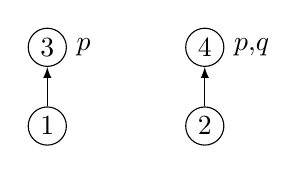
\begin{tikzpicture}[>=latex]
  \node (n1) at (0,0) [shape=circle,draw,inner sep=2pt, label=right:$$] {$1$} ;
  \node (n2) at (2,0) [shape=circle,draw,inner sep=2pt, label=right:$$] {$2$} ;
  \node (n4) at (0,1) [shape=circle,draw,inner sep=2pt, label=right:$p$] {$3$} ;
  \node (n5) at (2,1) [shape=circle,draw,inner sep=2pt, label=right:$p{,}q$] {$4$} ;
  \draw [->] (n1) -- (n4);
  \draw [->] (n2) -- (n5);
\end{tikzpicture}
\end{center}
%
where $\rg\ l=\cset{p,q}$ and the valuation is defined as
$l(3)=\cset{p}, l(4)=\cset{p,q}, l(1)=l(2)=\cset{}$. The initial values of $S$ and $F$ are
shown in Table~\ref{tab:example}.

\begin{table}[ht]
\centering
{\footnotesize
\begin{tabular}{|c|c|c|c|c|}
\hline
&\multicolumn{2}{|c|}{Initial}&\multicolumn{2}{|c|}{Final}\\
$v$ & $S(v)$ & $F(v)$ & $S(v)$&$F(v)$\\
\hline
$1$ & $\{1,2,3,4\}$ & $\top$ & $\{1,2\}$&$\top\wedge\diam p$\\
$2$ & $\{1,2,3,4\}$ & $\top$ & $\{2\}$&$\top\wedge\diam(p\wedge q)$\\
$3$ & $\{3,4\}$ & $p$ & $\{3,4\}$ &$p$\\
$4$ & $\{4\}$ & $p\wedge q$ & $\{4\}$&$p\wedge q$\\
\hline
\end{tabular}
\caption{Initial and final values of $F$ and $S$}\label{tab:example}
}
\end{table}

Suppose the following execution:
\begin{enumerate}
\item Choose $u=2,v=4,w=1$: detect that $1$ does not simulate $2$; set $S(2)=\{2,3,4\}$ and $F(2)=\top\wedge\diam(p\wedge q)$
\item Choose $u=2,v=4,w=3$: detect that $3$ does not simulate $2$; set $S(2)=\{2,4\}$ and $F(2)=\top\wedge\diam(p\wedge q)$
\item Choose $u=2,v=4,w=4$: detect that $4$ does not simulate $2$; set $S(2)=\{2\}$ and $F(2)=\top\wedge\diam(p\wedge q)$
\item Choose $u=1,v=3,w=3$: detect that $3$ does not simulate $1$; set $S(1)=\{1,2,4\}$ and $F(1)=\top\wedge\diam p$
\item Choose $u=1,v=3,w=4$: detect that $4$ does not simulate $1$; set $S(1)=\{1,2\}$ and $F(1)=\top\wedge\diam p$
\end{enumerate}
After the fifth iteration it terminates. The final output is shown
in Table~\ref{tab:example}. From this output one may conclude that,
since $\simset_\subseteq(4)=\{4\}$, node $4$ has an \posre, namely
$p\wedge q$. Node $2$ also has the \EL-RE $\top\wedge\diam(p\wedge
q)$. In contrast $3$ does not have an \EL-RE because every
$\pos$-formula true at $3$ is also true at $4$ (in this case, the
only such possible formula is $p$ itself, or logically equivalent
formulas such as $\top\wedge p\wedge p$). Nor $3$ has an \posre.
\end{ex}
\fi

\iffullversion
\begin{theorem}\label{thm:correctness-schematic-GRE}
Let $S$ and $F$ be the output of the Algorithm
\ref{alg:schematic-GRE} with input $\gG=\tup{N,\to,l}$. Then for each
node $v\in N$, $\interp{F(v)} = S(v) = \simset_\subseteq(v)$
\end{theorem}
\fi

\iffullversion
\begin{proof}
It is clear that for each node $v\in N$,
$\simset_\subseteq(v)=S(v)$. For the second part, we propose the
following invariant for the main loop:
\begin{itemize}
\item[$I_1$:] for each $v\in N$, $v \in \interp{F(v)}$
\item[$I_2$:] for each $u,v\in N$, $\interp{F(u)} \subseteq S(u)$
\end{itemize}
Let us analyze the state after the initialization, before line~\ref{alg:line:loop-begin} is executed for the fist time. On the one
hand, it is clear that for any node $v\in N$, $v \in \interp{F(v)}$, so
$I_1$ is verified. On the other, if $v\notin S(u)$ then
$l(u)\not\subseteq l(v)$ and so there is a propositional symbol
$p$ such that $p \in l(u)$ and $p \notin l(v)$. Since $v\notin\interp{p}$
then $v\notin\interp{\bigwedge l(u)}$ and therefore
$v\notin \interp{F(u)}$.

Suppose that $I_1$ and $I_2$ are true before executing
line~\ref{alg:line:loop-body-begin}. For all $v\in N$ let $S(v)=S_v$ and
$F(v)=\phi_v$ in this state. Let $u,v,w$ be the chosen nodes. We
show that the invariant is reestablished after executing line
\ref{alg:line:loop-body-end-1}. Since $F$ and $S$ only change for $u$,
it suffices to show
\begin{itemize}
\item[$I_1'$:] $u \in \interp{\phi_u\wedge\diam \phi_v}$
\item[$I_2'$:] $\forall v\in N, \interp{\phi_u\wedge\diam \phi_v} \subseteq S_u\setminus\{w\}$
\end{itemize}
For $I_1'$, it is clear from $I_1$ that $u \in \interp{\phi_u}$ and
$v \in \interp{\phi_v}$. Since $u\to v$ we conclude $u \in \interp{\diam
\phi_v}$.

For $I_2'$ we show that for any $v$, if $v\notin S_u\setminus\{w\}$
then $v\notin \interp{\phi_u\wedge\diam \phi_v}$. If $v\notin S_u$,
by $I_2$ we know $v\notin \interp{\phi_u}$ and therefore $v\notin
\interp{\phi_u\wedge\diam \phi_v}$. Suppose $v=w$ and, by
contradiction, assume $v \in \interp{\phi_u\wedge\diam \phi_v}$.
Then there is $w'\in N$ such that $v\to w'$ and $w' \in
\interp{\phi_v}$. By $I_2$ this implies $w'\in S_v$. Hence
$w'\in\su(w)\cap S_v$ and this contradicts the choice of $u,v,w$.

When the algorithm terminates, $S=\simset_\subseteq$ and therefore
the invariant $I_2$ implies that for each $u,v\in N$,
$F(u) \subseteq \simset_\subseteq(u)$. On the other hand, $I_1$
implies that $u \in \interp{F(u)}$ and by Proposition \ref{prop:equiv} we
have that if $v\in \simset_\subseteq(u)$ then $v \in \interp{F(u)}$.
Therefore for each $u,v\in N$, $\interp{F(u)} = \simset_\subseteq(u)$. So defining $\form:=F$ we obtain the desired result.
\end{proof}
\else
\fi

\iffullversion
\begin{theorem}
Algorithm~\ref{alg:schematic-GRE} with input $\gG = \tup{N,\to,l}$
terminates in time
$O(\size{{\to}}^2\cdot\size{N}^3+\size{N}\cdot\size{\rg\ l})$.
\end{theorem}
\fi

\iffullversion
\begin{proof}
For a naive implementation, the main loop executes at most
$\size{N}^2$ may times and to find $u,v,w$ in
line~\ref{alg:line:loop-begin} we need $O(\size{N}\cdot\size{{\to}}^2)$
many steps. The running time of the loop body is absorbed by this
last quantity. Hence, in total, the execution time of the main loop
is $O(\size{{\to}}^2\cdot\size{N}^3)$. For each $v\in N$, we need
$O(\size{\rg\ l})$ many steps for lines~\ref{alg:line:init1} and~\ref{alg:line:init2}. So in total, the initialization takes
$O(\size{N}\cdot\size{\rg\ l})$ many steps.
\end{proof}
\else
\fi

\iffullversion
\begin{algorithm} \small
\io

\ForEach{$v\in \Delta$}{ $\prevS(v):=\Delta$

\If{for all binary $r$, $\su{r}{v}=\emptyset$}{$S(v):=\{u\in \Delta
\mid \unary(v)\ \subseteq \unary(u) \}$

$F(v):=\bigwedge\unary(v)$ } \Else{ let $r$ be a binary relation
such that $\su{r}{v}\not=\emptyset$

 $S(v):=\{u\in \Delta \colon
\unary(v) \subseteq \unary(u)\wedge\su{r}{u}\not=\emptyset \}$

$F(v):=\diam\top\wedge\bigwedge P(v)$ }}

\While{$\exists\ v\in \Delta:S(v)\not=\prevS(v)$}{

$\{\ I_1:\mbox{\bf assert\ }(\forall v)\ S(v)\subseteq\prevS(v)\ \}$

$\{\ I_2:\mbox{\bf assert\ }(\forall r,u,v,w)\
[(u,v)\in\interp{r}\wedge w\in
S(u)]\Rightarrow[\su{r}{w}\cap\prevS(v)\not=\emptyset]\ \}$

\ForEach{\mbox{\rm binary relation $r$ and $u\in \pr{r}{v}$}}{

$remove := \pr{r}{\prevS(v)}\setminus\pr{r}{S(v)}$

$S(u):=S(u)\setminus remove$

\If{$\diam F(v)$ is not a conjunct of $F(u)$}{ $F(u):=F(u)\wedge
\diam F(v)$\label{alg:line:loop-body-end-2} } }

$\prevS(v)=S(v)$

} \caption{\small refined $\EL$-similarity and
\posre}\label{alg:refined-GRE}
\end{algorithm}
\fi

Algorithm \ref{alg:schematic-GRE} can be easily modified to
calculate the \ELAN-RE of each simulator set $\simset_{\ELAN}$ by
adjusting the initialization: replace $\subseteq$ by $=$ in the
initialization of $S(v)$ and initialize $F(v)$ as
$\bigwedge\left(\unary(v)\cup\overline \unary(v)\right)$,
where $\overline \unary(v)=\{\lnot p\mid v\notin\interp{p}\}$.


With a naive implementation Algorithm~\ref{alg:schematic-GRE}
executes in time $O(\size{\Delta}^3\times$
$\size{\interp{\cdot}}^2)$
%\fixme{Santi: chequear la complejidad}
providing a polynomial solution to the \EL and \ELAN-GRE problems.
Algorithm~\ref{alg:schematic-gen-sim} can be transformed to run with a lower complexity
as in shown in~\cite{HHK95}; moreover this version of the algorithm can be adapted to
compute \EL- and \ELAN-RE for an arbitrary subset of the domain of $\tup{\Delta,\interp{\cdot}}$
 in $O(\size{\Delta}\times\size{\interp{\cdot}})$ steps. We shall skip the details.


%Given $\gG = \tup{N,\to,l}$,
%the
%
%$F$, the set of \posre, and $S$, the simulator sets s.t.\ $(\forall
%v\in \Delta)\ \interp{F(v)}=S(v)=\simset_\EL(v)$

%
\begin{theorem}\label{thm:complexity-EL-GRE}
The \EL and \ELAN-GRE problems over $\gM=\tup{\Delta,\interp{\cdot}}$ have complexity
$O(\size{\Delta}\times\size{\interp{\cdot}})$.
\end{theorem}

Theorem~\ref{thm:complexity-EL-GRE} answers a question left open
in~\cite{AKS08}: the \EL-GRE problem can be solved in polynomial
time. Note, however, that this  result assumes a convenient representation of
formulas like, for example, directed acyclic graphs, to ensure that
each step of the formula construction can be done in $O(1)$. In
\sect{size} we will take a closer look at the issue and its relation to
the size of the smallest $\+L$-RE.


%Theorem~\ref{thm:complexity-EL-GRE} shows that there are efficient
%GRE algorihtms for \EL and \ELAN; languages which are --as discussed
%in \sect{choosinglanguage}-- generally simple to realize. The
%methods presented here, together with previous results
%of~\cite{AKS08} indicate that algorithms for computing
%$\+L$-simulator sets can, in many cases, be adapted to solve the
%$\+L$-GRE problem at no extra complexity cost.


Algorithm~\ref{alg:schematic-GRE} was obtained by adding formula annotations
to a standard `\EL-simulation-minimization' algorithm. Given an
$\+L$-simulation-minimization, we can typically adapt it in an analogous
way to obtain an $\+L$-GRE algorithm.
The obtained algorithm computes $\+L$-REs for \emph{every} element of the
domain simultaneously.
This will make it particularly suitable for applications with
static domains requiring references to many objects.
% but given its low complexity
%and the fact that termination is ensured (no risk of infinite regression, see~\cite{dale91:_gener_refer_expres_invol_relat}),
%it seems suitable for most applications.
 Moreover, the algorithm can be adapted
to dynamic domains by using techniques used to recompute simulations (see~\cite{saha:incre07}),
so that only those RE that were affected by a change in the domain need to be
recomputed.

We have not addressed so far other relevant issues of the
GRE problem besides computational complexity. In particular,
Algorithm~\ref{alg:schematic-GRE} pays no attention to the use of
preferences among relations when generating an RE (i.e., preferring
the selection of certain attributes over others, when possible).
While there is room for improvement (e.g., making a weighted choice
instead of the non-deterministic choice when choosing elements
in the main loop of the algorithm), support for preferences is not
one of the strong points of this family of algorithms.
We consider algorithms with strong support for preferences in the following section.

\newcommand{\instFun}[2]{\texttt{#1}\ensuremath{_{#2}}\xspace}

\section{GRE via Building Simulated Models}\label{sec:krahmer}

Krahmer~et~al.~\cite{Krahmer2003} introduce an algorithm for
content determination based on the computation of \emph{subgraph isomorphisms}.
It is heavily regulated by cost functions and is therefore apt to implement
different preferences. In fact, they show that using suitable cost functions it
can simulate most of the previous proposals. Their algorithm takes as input
a labeled directed graph $G$ and a node $e$ and returns, if possible,
a connected subgraph $H$ of $G$, containing $e$ and enough edges to
distinguish $e$ from the other nodes.

In this section we will identify its
underlying notion of expressiveness and  will extend it to accommodate other notions.
To keep the terminology of~\cite{Krahmer2003}, in what follows
we may alternatively talk of \emph{labeled graphs} instead of relational
models. The reader should observe that they are essentially the same
mathematical object, but notice that in~\cite{Krahmer2003},  propositions are encoded using
looping binary relations (e.g., they write $\nDog(e,e)$ instead of $\nDog(e)$).

The main ideas of their algorithm can be
intuitively summarized as follows.
Given two labeled graphs $H$ and $G$, and vertices $v$ of $H$
and $w$ of $G$, we say that the pair $(v,H)$ {\em refers}
to the pair $(w,G)$ iff $H$ is connected and $H$ can be ``placed
over'' $G$ in such a way that: 1) $v$ is placed over $w$; 2) each
node of $H$ is placed over a node of $G$ with at least the same
unary predicates (but perhaps more); and 3) each edge from $H$ is
placed over an edge with the same label. Furthermore, $(v,H)$ {\em
uniquely refers} to $(w,G)$ if $(v,H)$ refers to $(w,G)$ and there
is no vertex $w'\not=w$ in $G$ such that $(v,H)$ refers to $(w',G)$.
The formal notion of a labeled graph being ``placed over'' another
one is that of {\em subgraph isomorphism}:
$H=\tup{\Delta_H,\interp{\cdot}_H}$ can be placed over
$G$ iff there is a labeled subgraph (i.e., a graph obtained from
$G$ by possibly deleting certain nodes, edges, and propositions from some nodes)
$G'=\tup{\Delta_{G'},\interp{\cdot}_{G'}}$ of $G$ such that $H$ is {\em
isomorphic} to $G'$, which means that there is a
bijection $f:\Delta_{H}\to\Delta_{G'}$ such that for all vertices
$u,v\in \Delta_H$, $u\in\interp{p}_{H}$ iff $f(u)\in\interp{p}_{G'}$
and $(u,v)\in\interp{r}_{H}$ iff $(f(u),f(v))\in\interp{r}_{G'}$.
%
\begin{figure}
\centering
\begin{tabular}{c@{\hspace{1.0cm}}c@{\hspace{1.0cm}}c@{\hspace{1.0cm}}c}
\begin{picture}(22,50)
\put(0,0){\begin{tikzpicture}
  [
    n/.style={circle,fill,draw,inner sep=1.5pt,node distance=1.5cm},
    aSniffing/.style={->, >=stealth, semithick, shorten <= 3pt, shorten >= 3pt},
  ]
 \node[n,label=above:$v$,label=below:{\relsize{-1}$\begin{array}{c}\nDog\\\ \end{array}$}] (a) {};
 \end{tikzpicture}}
 \end{picture}
&
\begin{picture}(55,50)
\put(0,0){\begin{tikzpicture}
  [
    n/.style={circle,fill,draw,inner sep=1.5pt,node distance=1.5cm},
    aSniffing/.style={->, >=stealth, semithick, shorten <= 3pt, shorten >= 3pt},
  ]
 \node[n,label=above:,label=below:{\relsize{-1}$\begin{array}{c}\ \end{array}$}] (a) {};

 \node[n,label=above:$v$,label=below:{\relsize{-1}$\begin{array}{c}\nDog\\\ \end{array}$}, right of=a] (b) {};

 \draw [aSniffing,bend right=40] (b) to node[auto,swap]{\relsize{-1}$\aSniffing$} (a);

 \end{tikzpicture}}
 \end{picture}
&
\begin{picture}(70,50) \put(0,0){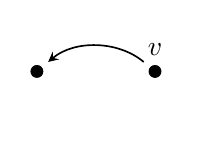
\begin{tikzpicture}
  [
    n/.style={circle,fill,draw,inner sep=1.5pt,node distance=1.5cm},
    aSniffing/.style={->, >=stealth, semithick, shorten <= 3pt, shorten >= 3pt},
  ]
 \node[n,label=above:,label=below:{\relsize{-1}$\begin{array}{c}\nDog\end{array}$}] (a) {};

 \node[n,label=above:$v$,label=below:{\relsize{-1}$\begin{array}{c}\nDog\\ \aSmall \end{array}$}, right of=a] (b) {};

 \draw [aSniffing,bend right=40] (b) to node[auto,swap]{\relsize{-1}$\aSniffing$} (a);

 \end{tikzpicture}}
 \end{picture}
&
\begin{picture}(77,50)
\put(0,0){\begin{tikzpicture}
  [
    n/.style={circle,fill,draw,inner sep=1.5pt,node distance=1.5cm},
    aSniffing/.style={->, >=stealth, semithick, shorten <= 3pt, shorten >= 3pt},
  ]
 \node[n,label=above:$v$,label=below:{\relsize{-1}$\begin{array}{c}\nDog\end{array}$}, right of=a] (b) {};
%
 \node[n,label=above:,label=below:{\relsize{-1}$\begin{array}{c}\nCat\\ \aSmall\end{array}$}, right of=b] (c) {};
%
 \draw [aSniffing,bend right=40] (c) to node[auto,swap]{\relsize{-1}$\aSniffing$} (b);
 \end{tikzpicture}}
 \end{picture}
% %
% \begin{picture}(77,50)
% \put(0,0){\begin{tikzpicture}
%   [
%     n/.style={circle,fill,draw,inner sep=1.5pt,node distance=1.5cm},
%     aSniffing/.style={->, >=stealth, semithick, shorten <= 3pt, shorten >= 3pt},
%   ]
%  \node[n,label=above:,label=below:{\relsize{-1}$\begin{array}{c}\end{array}$}] (a) {};
%
%  \node[n,label=above:$v$,label=below:{\relsize{-1}$\begin{array}{c}\end{array}$}, right of=a] (b) {};
%
%  \draw [aSniffing,loop left] (a) to node[above,xshift=-5pt]{\relsize{-1}$\aSniffing$} (a);
%
%  \draw [aSniffing,bend right=40] (b) to node[auto,swap]{\relsize{-1}$\aSniffing$} (a);
%  \end{tikzpicture}}
%  \end{picture}
\vspace{-.2cm}\ \\
(i)&(ii)&(iii)&(iv)
\end{tabular}
 \caption{Some connected subgraphs $(v,H)$ of scene $\+S$ in Figure~\ref{fig:cat-dog-1}.\label{fig:subgraphs}}
 \end{figure}

As an example, consider the relational model depicted in
Figure~\ref{fig:cat-dog-1} as a labeled graph $G$, and let us
discuss the pairs of nodes and connected subgraphs $(v,H)$ shown in
Figure~\ref{fig:subgraphs}. Clearly, (i) refers to the pair $(w,G)$
for any node $w\in\{a,b,d\}$; (ii) refers to $(w,G)$ for
$w\in\{b,d\}$; and both (iii) and (iv) uniquely refer to $(b,G)$. Notice
that (i)--(iv) can be respectively realized as ``{\em a dog}'',
``{\em a dog that sniffs something}'', ``{\em a small dog that
sniffs a dog}'' (cf. $\gamma_1$ in Table~\ref{tab:gammas}) % and ``{\em
% something that
% sniffs something else that sniffs itself}''.
and ``{\em the dog that is sniffed by a small cat}'' (cf.~$\gamma_4$ in
Table~\ref{tab:gammas}).


% For reasons of space we assume the reader is familiar with this
% algorithm and refer her to that article for further
% information.\fxnote{\tiny Intentemos depender lo menos posible del
% articulo de Krahmer.  En todo caso, dar una idea intuitiva del
% approach antes de decir esto.  Tenemos todavia una pagina. }



% \fxnote{\tiny Reescribir los siguientes dos parrafos. Decir algo como, 'once
% more we'll try to remain as close as possible to the algorithms of the original
% article and we will then start by pointing out the differences with the algorithms
% we presented in the previous section'}

It is important to emphasize that there is a substantial difference
between the algorithm presented in~\cite{Krahmer2003} and the one we discussed
in the previous sections:
%
% First note that scenes are encoded in that article in a slightly
% different way: there, graphs have only labels on edges, and
% non-relational attributes such as \emph{type} or \emph{color} are
% represented by loops (e.g., $\aSmall(a,a)$). % \fxnote{\tiny Aca decia
% `While our presentation is, arguably, conceptually cleaner, it
% forces us to treat the atomic and relational cases separately'. No
% hablemos de `our presenation' respecto de la de la seccion anterior.
% O ninguna o las dos son `our presentation'. }
%
while the input is a labeled graph $G$ and a target node $v$, the
output is, in this case (and unlike the definition of $\+L$-GRE problem
presented in \sect{technical} where the output is a {\em formula}), the cheapest (with
respect to some, previously specified cost function) connected
{\em subgraph} $H$ of $G$ which uniquely refers to $(v,G)$ if there is
such $H$, and $\bot$ otherwise.

We will not deal with cost functions here; it is enough to know
that a cost function is a monotonic function that assigns to each
subgraph of a scene graph a non-negative number which expresses the
goodness of a subgraph --e.g.\ in Figure~\ref{fig:subgraphs}, one
may tune the cost function so that (iii) is cheaper than (iv), and hence
(iii) will be preferred over (iv).
%By defining cost functions in
%different ways, \cite{Krahmer2003} shows that it is possible to mimic various algorithms for the
%generation of referring expressions known from the literature.

For reasons of space we will not introduce here the detailed algorithm proposed
in~\cite{Krahmer2003}. Roughly, it is a
straightforward branch and bound algorithm that systematically tries all
relevant subgraphs $H$ of $G$ by starting with the subgraph
containing only vertex $v$ and expanding it recursively by trying to
add edges from $G$ that are adjacent to the subgraph $H$ constructed
up to that point. In the terminology
of~\cite{Krahmer2003} a {\em distractor} is a node of $G$ different from
$v$ that is also referred by $H$.
The algorithm ensures that a subgraph uniquely refers to the
target $v$ when it has no distractors. Reached this point we
have a new candidate for the solution, but there can be other
cheaper solution so the search process continues until the
cheapest solution is detected. Cost functions are used to
guide the search process and to give preference to some solutions
over others.
% In the definition of~\cite{Krahmer2003}, $H$ is  such that every \emph{subgraph isomorphism}
% $f$ between $H$ and $G$ (i.e., every isomorphism between $H$
%  and a subgraph of $G$)
%  satisfies $f(u) = u$.
%

Here is the key link between the graph-based method
of~\cite{Krahmer2003} and our logical-oriented perspective: on
finite relational models, subgraph isomorphism corresponds to
\EPFOL-simulations, in the sense that given two nodes $u,v$ of
$G$, there is a subgraph isomorphic to $G$ via $f$, containing $u$ and
$v$, and such that $f(u)=v$ iff $u \simul{\+\EPFOL} v$.
%
Having made explicit this notion of sameness and, with it, the
logical language associated to it, we can proceed to generalize the
algorithm to make it work for other languages, and to adapt it in
order to output a formula instead of a graph. This is shown in
Algorithms~\ref{alg:makeRE} and~\ref{alg:find}.
%
\begin{center}\begin{minipage}[t]{5.1cm}%
\begin{algorithm}[H]\small
\SetKwFunction{makeRE}{makeRE$_\+L$}
\SetKwFunction{findGraph}{find$_\+L$}
\SetKwFunction{init}{init_$\+L$}
\SetKwFunction{buildF}{buildF$_\+L$}

\caption{\small \texttt{makeRE}$_\+L$($v$)}\label{alg:makeRE}

%$v_H$ := \emph{new node}\;

\SetKwInOut{Input}{input}\SetKwInOut{Output}{output}
\Input{an implicit finite $G=\tup{\Delta_G,\interp{\cdot}}$ and $v\in\Delta_G$}
\Output{an $\+L$-RE for $v$ in $G$ if there is one, or else $\bot$}
\BlankLine

\vspace{3.0pt}

\BlankLine

$H$ := $\tup{\cset{v},\emptyset}$\; $f$ := $\cset{v \mapsto v}$\;
$H'$ := \findGraph($v, \bot, H, f$)\;
\BlankLine
\Return{\buildF$(H',v)$}\;
\end{algorithm}
  \end{minipage}
\hspace{.05cm}
  \begin{minipage}[t]{6.8cm}%
\begin{algorithm}[H] \small
\SetKwFunction{findGraph}{find$_\+L$} \SetKwFunction{cost}{cost}
\SetKwFunction{matchGraph}{match$_\+L$}
\SetKwFunction{extendGraph}{extend$_\+L$}


\caption{\small \texttt{find}$_\+L$($v, \mathit{best},
H,f$)}\label{alg:find}

\If{$\mathit{best} \neq \bot \land \cost(\mathit{best}) \leq
\cost(H)$}{\Return $\mathit{best}$} $\mathit{distractors}$ :=
$\cset{n \mid n \in \Delta_G, n \neq v , v \simul{\+L} n}$\;
\If{$\mathit{distractors} = \emptyset$}{\Return $H$}
\ForEach{$\tup{H',f'} \in \extendGraph(H,f)$}{
  $I$ := \findGraph($v,\mathit{best},H', f'$)\;
  \If{$\mathit{best} = \bot \lor \cost(I) \leq \cost(\mathit{best})$}{$\mathit{best} := I$}
} \Return{$\mathit{best}$}\;
\end{algorithm}
  \end{minipage}%
\end{center}
%
These algorithms are parametric on $\+L$; to make them concrete, one
needs to provide appropriate versions of \instFun{buildF}{\+L} and
\instFun{extend}{\+L}. The former transforms the computed {\em
graph} which uniquely refers to the target $v$ into an $\+L$-RE {\em
formula} for $v$; the latter tells us how to extend $H$ at each step
of the main loop of Algorithm~\ref{alg:find}. Note that, unlike the
presentation of~\cite{Krahmer2003}, \instFun{makeRE}{\+L} computes
not only a graph $H$ but also an $\+L$-simulation $f$. %%
%
% \begin{algorithm}\small
% \SetKwFunction{makeRE}{makeRE$_\+L$}
% \SetKwFunction{findGraph}{find$_\+L$}
% \SetKwFunction{init}{init_$\+L$}
% \SetKwFunction{buildF}{buildF$_\+L$}
%
% \caption{\small \texttt{makeRE}$_\+L$($v$)}\label{alg:makeRE} $v_H$
% := \emph{new node}\; $\tup{H,f}$ :=
% $\tup{\tup{\cset{v_H},\emptyset,\emptyset}, \cset{v_H \mapsto v}}$\;
% $H'$ := \findGraph($v_H, \bot, H, f$)\;
% \Return{\buildF($H',v_H$)}
% \end{algorithm}
%
%
% \begin{algorithm} \small
% \SetKwFunction{findGraph}{find$_\+L$} \SetKwFunction{cost}{cost}
% \SetKwFunction{matchGraph}{match$_\+L$}
% \SetKwFunction{extendGraph}{extend$_\+L$}
%
%
% \caption{\small \texttt{findGraph}$_\+L$($v_H, \mathit{best}, H,f$)}
%
% \If{$\mathit{best} \neq \bot \land \cost(\mathit{best}) \leq
% \cost(H)$}{\Return $\mathit{best}$} $\mathit{distractors}$ :=
% $\cset{n \mid n \in \Delta_G \land n \neq v \land v_H \simul{\+L}
% n}$\; \If{$\mathit{distractors} = \emptyset$}{\Return $H$}
% \ForEach{$\tup{H',f'} \in \extendGraph(H,f)$}{
%   $I$ := \findGraph($v_H,\mathit{best},H', f'$)\;
%   \If{$\mathit{best} = \bot \lor \cost(I) \leq \cost(\mathit{best})$}{$\mathit{best} := I$}
% } \Return{$\mathit{best}$}
% \end{algorithm}
%
%
In order to make the discussion of the differences with the original
algorithm simpler, we analyze next the case $\+L=\EPFOL$ and $\+L=\EL$.

% \instFun{buildF}{\EPFOL}
% and \instFun{extend}{\EPFOL} in
% Algorithms~\ref{alg:build-form-epfol}
% and~\ref{alg:extend-epfol}.
%
%
\paragraph{The case of $\EPFOL$.} From the computed cheapest isomorphic
subgraph $H'$ one can easily build an \EPFOL-formula that uniquely
describes the target $v$, as is shown in
Algorithm~\ref{alg:build-form-epfol}. Observe that if
$\FOL$-simulations were used instead, we would have to include also
which unary and binary relations \emph{do not hold} in $H'$.
%
\begin{center}\begin{minipage}[t]{6.3cm}%
\begin{algorithm}[H]\small
\caption{\small
\texttt{buildF}$_\EPFOL(H',v)$}\label{alg:build-form-epfol}
\textbf{let}
$H' = \tup{\cset{a_1\ldots a_n}, \interp{\cdot}}$,$v=a_1$\;
%\tcp{let $v=a_1$}
$\gamma$ := $\displaystyle \bigwedge_{\mathclap{a_i \neq a_j}} (x_i
\not\approx x_j) \land \bigwedge_{\mathclap{(a_i,a_j) \in
\interp{r}}} r(x_i,x_j) \land \bigwedge_{\mathclap{a_i \in
\interp{p}}}p(x_i)$

\BlankLine
\vspace{2.2pt}
\Return{$\exists x_2\ldots \exists x_n . \gamma$}\;
\end{algorithm}
\end{minipage}
\hspace{.2cm}
\begin{minipage}[t]{5.2cm}
\begin{algorithm}[H]\small
\SetKwFunction{extendGraph}{extend$_\EPFOL$}

\caption{\small
\texttt{extend}$_\EPFOL(H,f)$}\label{alg:extend-epfol}

 $A$ := $\cset{H {+} p(u) \mid u \in \Delta_H, $

 \hfill $u \in \interp{p}_G  \setminus \interp{p}_H}$\;

 $B$ := $\cset{H {+} r(u,v) \mid u \in \Delta_H, $

 \hfill $\{(u,v),(v,u)\}\cap \interp{r}_G \setminus \interp{r}_H\not=\emptyset}$\;

 \Return{$(A \cup B) \times \cset{\mathit{id}}$}\;
\end{algorithm}
\end{minipage}
\end{center}
%
Regarding the function which extends the given graph in all possible
ways (Algorithm~\ref{alg:extend-epfol}), since $H$
 is a subgraph of $G$, $f$ is the
trivial identity function $\mathit{id(x)} = x$. We will see the need
for $f$ when discussing the case of less expressive logics like \EL.
In \instFun{extend}{\EPFOL} we follow the notation
of~\cite{Krahmer2003} and write, for a relational model
$G = \tup{\Delta,
\interp{\cdot}}$,  $G + p(u)$ to denote the model $\tup{\Delta
\cup \cset{u},\interp{\cdot}'}$ such that $\interp{p}' = \interp{p}
\cup \cset{u}$ and $\interp{q}' = \interp{q}$ when $q \neq p$.
Similarly, $G + r(u,v)$ denotes the model $\tup{\Delta \cup
\cset{u,v},\interp{\cdot}'}$ such that $\interp{r}' = \interp{r}
\cup \{(u,v)\}$ and $\interp{q}' = \interp{q}$ when $q \neq r$. It
is clear, then, that this function is returning all the
\emph{extensions} of $H$ by adding a missing attribute or relation
to $H$, just like is done in the original algorithm.

\paragraph{The case of $\EL$.}
Observe that \instFun{find}{\EL} uses an \EL-simulation, and any
\EPFOL-simulation is an \EL-simulation.
%
One could, in principle, just use \instFun{extend}{\EPFOL} also for
\EL. If we do this, the result of \instFun{find}{\EL} will be a
subgraph $H$ of $G$ such that for every \EL-simulation $\sim$, $u
\sim v$ iff $u = v$. The problem is that this subgraph $H$ may
contain cycles and, as it is well known, \EL (even \ALC) are
incapable to distinguish a cycle from its {\em
unraveling}\footnote{Informally, the unraveling of $G$, is a new
graph, whose points are paths of $G$ from a given starting node.
That is, transition sequences in $G$ are explicitly represented as
nodes in the unraveled model. See~\cite{BRV01} for a formal
definition.}. Hence, although subgraph isomorphism get along with
$\EPFOL$, it is too strong to deal with \EL.
%
%
% was observed in \sect{technical}, they cannot be
% distinguished using \EL.\fxnote{\tiny Esto no queda superclaro en la
% seccion anterior. La referencia es vaga. Vale la pena contar esto?}
% The upshot is that we might be unable to realize the outcome of such
% function.

A well-known result establishes that every relational model $\+M$ is
equivalent, with respect to \EL-formulas,\footnote{Actually, the
result holds even for \ALC-formulas.} to the unraveling of $\+M$.
That is, any model and its unraveling satisfy exactly the same \EL-formulas.
% \fxnote{\tiny tendriamos que introducir mejor
% (intuitvamente) que es el unraveling. Ademas de depender de Khramer
% estamos haciendo cambios usando cosas que no definimos bien.  Esta
% parte es muy dificil de leer.}
 Moreover, the unraveling of $\+M$ is
always a tree, and as we show in Algorithm~\ref{alg:build-form-el},
it is straightforward to extract a suitable \EL-formula from a tree.

Therefore, we need \instFun{extend}{\EL} to return all the possible
``extensions'' of $H$. Now ``extension'' does not mean to be a
subgraph of the original graph $G$ anymore. We do this
by either adding a new proposition or a new edge
that is present in the unraveling of $G$ but not in $H$. This is
shown in Algorithm~\ref{alg:extend-el}.
%
\begin{center}\begin{minipage}{5cm}%
\begin{algorithm}[H] \small
\SetKwFunction{buildF}{buildF$_\EL$} \caption{\small
\texttt{buildF}$_\EL(H',v)$}\label{alg:build-form-el} \mbox{{\bf
requires} $H'$ to be a tree}

$\gamma$ := $\cset{\exists r.\buildF(H',u) \mid$

\hfill$ (v,u) \in \interp{r}}$\;

\Return{$ (\bigwedge\gamma) \land (\bigwedge_{v \in
\interp{p}}p)$}\;
\end{algorithm}
\end{minipage}
\begin{minipage}{7cm}%
\begin{algorithm}[H]\small
\SetKwFunction{extendGraph}{extend$_\EL$} \caption{\small
\texttt{extend}$_\EL(H,f)$}\label{alg:extend-el}

$A$ :=\\
\ \ \ \ \  $\cset{\tup{H {+} p(u),f} \mid u \in \Delta_H, u \in
\interp{p}_G \setminus \interp{p}_H}$\; $B$ := $\emptyset$\;
\ForEach {$u \in \Delta_G$}{
  \ForEach{$u_H \in \Delta_H / (f(u_h),u) \in \interp{r}_G$}{
    \If{$\forall v : (u_H,v) \in \interp{r}_H \Rightarrow f(v) \neq u$}{
      $n$ := \emph{new node}\;
      $B$ := $B \ \cup $

      \hfill $\cset{\tup{H + r(u_H,n),f \cup \{n \mapsto u\}}}$\;
    }
  }
  }
  \Return{$A \cup B$}\;
\end{algorithm}
\end{minipage}
\end{center}
%
Observe that the behavior of \instFun{find}{\EL} is quite sensible
to the {\tt cost}  function employed. For instance, on cyclic models,
a {\tt cost} function that does not guarantee the unraveling is explored in a
breadth-first way may lead to non-termination (since
\instFun{find}{\EL} may loop exploring an infinite branch).

%It is also possible to use modal model-theoretical results to put a
%bound check that avoids generating an unraveling of infinite depth
%when there is no possible referring expression, but we will not go
%into the details for reasons of space.\fxnote{\tiny No tiene
%suficiente detalle para que se entienda.  Extender.}


% \begin{algorithm}\small
% \SetKwFunction{extendGraph}{extend$_\EL$}
% \caption{\small \texttt{extend}$_\EL(H,f)$}\label{alg:extend-el}
%
% $a$ :=  $\cset{\tup{H {+} p(u),f} \mid u \in \Delta_H, u \in \interp{p}_G {-} \interp{p}_H}$\;
% $b$ := $\emptyset$\;
% \ForEach {$u \in \Delta_G$}{
%   \ForEach{$u_H \in \Delta_H / (f(u_h),u) \in \interp{r}_G$}{
%     \If{$\forall v . ((u_H,v) \in \interp{r}_H \Rightarrow f(v) \neq u)$}{
%       $n$ := \emph{new node}\;
%       $b$ := $b \cup \cset{\tup{H + r(u_H,n),f[n \mapsto u]}}$\;
%     }
%   }
%   }
%   \Return{$a \cup b$}
% \end{algorithm}


As a final note on complexity, although the set of \EL-distractors
may be computed more efficiently than \EPFOL-distractors (since
\EL-distractors can be computed in polynomial time, and computing
\EPFOL-distractors seems to require a solution to the subgraph
isomorphism problem which NP-complete), we cannot conclude that
\instFun{find}{\EL} is more efficient than \instFun{find}{\EPFOL} in
general: the model built in the first case may be exponentially
larger --it is an unraveling, after all. We will come back to this
in~\sect{size}.

\section{Combining GRE Methods}\label{sec:combining}

An appealing feature of formulating the GRE problem modulo expressivity
is that one can devise general strategies that combine $\+L$-GRE algorithms.
We illustrate this with an example.

The algorithms based on $\+L$-simulator sets like the ones in
\sect{simulation} simultaneously compute referring
expressions for every object in the domain, and do this for many
logics in polynomial time. This is an interesting property when one
anticipates the need of referring to a large number of elements.
However, this family of algorithms is not as flexible in terms of
implementing preferences as those we introduced in
\sect{krahmer} --though some flexibility can be obtained
by using cost functions for selecting $u$, $v$ and $w$ in the main
loop of Algorithm~\ref{alg:schematic-GRE} instead of the
non-deterministic choices.


There is a simple way to obtain an algorithm that is a compromise
between these two techniques. Let $A_1$ and $A_2$ be two procedures
that solve the $\+L$-GRE problem based on the techniques of
\sect{simulation} and~\sect{krahmer}, respectively.
One can first compute an $\+L$-RE for every possible object using
$A_1$ and then (lazily) replace the calculated RE for $u$ with
$A_2(u)$ whenever the former does not conform to some predefined
criterion. This is correct but we do better, taking advantage of the
equivalence classes obtained using $A_1$.

Since $A_1$ computes, for a given $\+M = \tup{\Delta,\interp{\cdot}}$, the
set $\simset(u)$ for every $u \in \Delta$, one can  build in polynomial time, using
the output of $A_1$, the model $\+M_{\+L} = \tup{\cset{[u] \mid u \in \Delta}, \interp{\cdot}_{\+L}}$,
such that:
$[u] = \cset{v \mid u \simul{\+L} v$ and $v \simul{\+L}
u}\quad \mbox{and}\quad \interp{r}_{\+L} = \cset{([u_1]\ldots [u_n])
\mid (u_1\ldots u_n) \in \interp{r}}$.
% $$
% \begin{array}{l@{\;=\;}l}
% \setlength{\abovedisplayskip}{0pt}%
% \setlength{\abovedisplayshortskip}{0pt}%
% [u] & \cset{v \mid u \simul{\+L} v \text{ and } v \simul{\+L} u}\\
% %\interp{p}_{\+L} &= \cset{[u] \mid u \in \interp{p}}\\
% \interp{r}_{\+L} & \cset{([u_1]\ldots [u_n]) \mid (u_1\ldots u_n) \in \interp{r}}
% \end{array}
% $$
$\+M_{\+L}$ is known as \emph{the $\+L$-minimization of $\+M$}. By a
straightforward induction on $\gamma$ one can verify that
$(u_1\ldots u_n) \in \interp{\gamma}$ iff $([u_1]\dots [u_n]) \in
\interp{\gamma}_{\+L}$ and this implies that $\gamma$ is an $\+L$-RE
for $u$ in $\+M$ iff it is an $\+L$-RE for $[u]$ in $\+M_{\+L}$.

If $\+M$ has a large number of indistinguishable elements (using $\+L$), then
 $\+M_{\+L}$ will be much smaller than $\+M$. Since the computational complexity of
 $A_2$ depends on the size of $\+M$, for very large scenes, one should compute
 $A_2([u])$ instead.

%
% \subsection{Incremental expressivity}
%
%It may appear from what we have discussed so far that one has to pick an expressivity $\+L$
%in advance and stick to it. That is not necessarily true.  Let $\+L_0$ be a sublanguage or $\+L_1$
%(e.g., \EL and \EPFOL, respectively) and assume one prefers $\+L_0$-REs, although for some
%elements of the domain $\+L_0$ may not be enough.

%In order to obtain a RE for an element $u$ in $\+M$, one can first try an $\+L_0$-GRE algorithm and
%obtain a formula $\gamma_0$. If $\interp{\gamma_0} = \cset{u}$ then we are done. If not, instead of
%finding a $\+L_1$-RE for $u$ in $\+M$, one can run a $\+L_1$-GRE algorithm for $u$ in
%$\+M_{\gamma_0}$, where $\+M_{\gamma_0}$\ldots\fixme{hace falta un algoritmo que calcule deltas}

\section{On the Size of Referring Expressions} \label{sec:size}

The expressive power of a language $\+L$ determines if there is an
$\+L$-RE for an element $u$. It also influences the \emph{size} of
the \emph{shortest} $\+L$-RE (when they exist). Intuitively, with
more expressive power we are able to `see' more differences and
therefore have more resources at hand to build a shorter formula.

A natural question is, then, whether we can characterize the relative size
of the $\+L$-REs for a given $\+L$. That is, if we can give (tight) upper
bounds for the size of the shortest $\+L$-REs for the elements of an arbitrary
model $\+M$, as a function of the size of $\+M$.

%\fixme{Incluir ejemplo de S/U y FO (Kams Result).}

For the case of one of the most expressive logics considered in this
article, \EPFOL, the answer follows from algorithm
\instFun{makeRE}{\EPFOL} in \sect{krahmer}. Indeed, if an
\EPFOL-RE exists, it is computed by \instFun{buildF}{\EPFOL}
from a model $H$ that is not bigger than the input model. It is easy
to see that this formula is linear in the size of $H$ and, therefore
the size of any \EPFOL-RE is $O(\size{\Delta} +
\size{\interp{\cdot}})$. It is not hard to see that this upper bound
holds for \FOL-REs too.% (cf.~\sect{krahmer} for details).

% Although \instFun{buildFormula}{\EL} also returns a formula that is linear
% in the size of the tree-model $H$, $H$ could be, in principle, exponentially
% larger than the input model. We can use this to give an exponential upper
% bound for the size of the shortest \EL-RE, but is it tight?

One is tempted to conclude from Theorem~\ref{thm:complexity-EL-GRE}
that the size of the shortest \EL-RE is $O(\size{\Delta} \times
\size{\interp{\cdot}})$, but there is a pitfall.
Theorem~\ref{thm:complexity-EL-GRE} assumes that formulas are
represented as a DAG and it guarantees that this DAG is polynomial
in the size of the input model. One can easily reconstruct
 (the syntax tree of) the formula from the DAG, but this, in principle, may lead
 to a exponential blow-up --the result will be an exponentially larger formula,
 but composed of only a polynomial number of different subformulas.
%
As the following example shows, it is indeed possible to obtain an \EL-formula
that is exponentially larger when expanding the DAG representation
generated by Algorithm~\ref{alg:schematic-GRE}.


%Is there an {\em intrinsic} gain in the succinctness of \ALC over
%\EL (or \ELAN over \EL)?
%More formally, is there a sequence of finite pointed models
%$(\+M_i,v_i)_{i\in\NN}$ such that for all $i$, if $n_i$ is the size
%of $\+M_i$, the shortest \EL-RE for $v_i$ has size at least say
%$2^{n_i}$ but $v_i$ has a \ALC-RE of size, say $O(n_i)$? We
%conjecture that the answer is yes, though the models $\+M_i$ seem to
%be far from simple to define.

%Of course, neither Algorithm \ref{alg:schematic-GRE} nor the more
%efficient implementations of it leading to the time complexity
%bounds of Theorem \ref{thm:complexity-EL-GRE} ensures us to obtain
%the shortest (or one of the shortest, in case there is more than
%one) \EL-RE. Forcing the algorithm to obtain the shortest referring
%expression (or at least one which is not is exaggeratedly large),
%seems to be much harder and still needs to be studied. For now, the
%following examples illustrate that the non-deterministic choices of
%$u$, $v$ and $w$ in the guard of the while loop of Algorithm
%\ref{alg:schematic-GRE} are quite sensitive to the size of the
%produced \EL-REs.

%We show that, over the same input $\gM=\tup{\Delta,\interp{\cdot}}$
%where $\size{\Delta}=n$, the $\EL$-REs output by Algorithm
%\ref{alg:schematic-GRE} may be of size greater than $2^n$ or of size
%$O(n^2)$, depending on these non-deterministic choices.

%Before going to the examples, it is important to make the following
%remark. All the computed $\EL$-RE $F(v)$ of Algorithm
%\ref{alg:schematic-GRE} may be stored in a polynomially bounded
%directed acyclic graph. This means that although $F(v)$ may have
%exponential size, the number of distinct subformulas of $F(v)$ is a
%polynomial of the size of the input $\+M$.
%Therefore, the time
%complexity bound of Theorem \ref{thm:complexity-EL-GRE} does not
%suppose a textual output of the referring expressions, but a
%compacted one (represented in a DAG).

%Fist, let us see an execution of Algorithm~\ref{alg:schematic-GRE}
%which outputs a \EL-RE of exponential size.

\begin{example}\label{ex:bad-length}
Consider a language with only one binary relation $r$, and let
$\gM=\tup{\Delta,\interp{\cdot}}$ where $\Delta=\{1,2,\dots, n\}$
and $(i,j)\in\interp{r}$ iff $i<j$.
Algorithm~\ref{alg:schematic-GRE} initializes $F(j)=\top$ for all
$j\in \Delta$. Suppose the following choices in the execution: For
$i=1,\dots, n-1$, iterate $n-i$ times picking $v=w=n-i+1$ and
successively $u=n-i,\dots, 1$. It can be shown that each time a
formula $F(j)$ %($1\leq j<n$)
 is updated, it changes from $\phi$ to
$\phi\wedge\diam\phi$ and hence it doubles its size.
Since $F(1)$ is updated $n-1$ many times, the size of $F(1)$ is
greater than $2^n$.

\iffullversion Suppose that in the first $n-1$ iterations we
successively choose $v=w=n$ and $u=n-1,n-2,\dots,1$. That is, we
discover that $n$ does not simulate $n-1,n-2,\dots,1$. We end up
with $F(1)=\dots=F(n-1)=\top\wedge\diam\top$ and
$S(1)=\dots=S(n-1)=W\setminus\{n\}$. Suppose that in the following
$n-2$ iterations we successively choose $v=w=n-1$ and
$u=n-2,n-3,\dots,1$, namely, we discover that $n-1$ does not
simulate $n-2,\dots,1$. We end up with
$F(i)=(\top\wedge\diam\top)\wedge \diam(\top\wedge\diam\top)$ and
$S(i)=\Delta\setminus\{n,n-1\}$, for $1 \le i \le n-1$. Following
this choice scheme, each time $F(1)$ is updated, it changes from
$\varphi$ to $\varphi\wedge\diam\varphi$. Since $F(1)$ is updated
$n-1$ many times, the size of $F(1)$ is
$O(2^n)=O(2^{\size{\Delta}})$. \fi
\end{example}

The large $\EL$-RE of Example~\ref{ex:bad-length} is due to an
unfortunate (non-deterministic) choice of elements.
Example~\ref{ex:not-that-bad-length} shows that another execution
 leads to a quadratic RE (but notice the
shortest one is linear: $(\exists r)^{(n-1)}.\top$).

\begin{example}\label{ex:not-that-bad-length}
%Let $\gM$ be the model of Example~\ref{ex:bad-length}.
Suppose now that in the first $n-1$ iterations we successively
choose $v=w=n-i$ and $u=v-1$ for $i=0\dots n-2$. It can be seen that
for further convenient choices, $F(1)$ is of size
$O(n^2)$.%
%
%
%We end up with $F(n)=\top$ and $F(i)=\top\wedge\diam F(i+1)$ for
%$i=1,\dots,n-1$. Up to this point, the size of $F(1)$ is linear in
%$n$. Of course, the algorithm does not stop here, but the reader can
%verify that if we successively choose $u=1$ and $v=w=n,n-1,\dots,2$
%we end up with $F(1)$ of size $O(n^2)$.
\end{example}

But is it always possible to obtain an \EL-RE of size polynomial in
the size of the input model, when we represent a formula as a
string, and not as a DAG? In~\cite{FG10} it is shown that the answer
is `no': for $\+L\in\{\ALC, \EL ,\ELAN\}$, the lower bound for the
length of the $\+L$-RE is exponential in the size of the input
model\footnote{
  More precisely, there are infinite models $G_1,G_2,\dots$ such that for
  every $i$, the size of $G_i$ is linear in $i$ but the size of the minimum RE
  for some element in $G_i$ is bounded from below by a function which is exponential
  on $i$.
}, and this lower bound is tight.

%Therefore, Theorem~\ref{thm:complexity-EL-GRE} is true {\em provided
%that $\+L$-formulas are represented as a DAG} (or other similar
%structures) but not as a plain string. This contraposition with
%respect to the representation shows that those relational models
%with target object which are exclusively referenced with
%$\+L$-formulas of exponential size are somewhat redundant.

% \fxnote{\tiny Include here new results?  Cite AiML?}
% We are yet unable to answer whether the exponential bound for the
% size of the minimum \EL-RE is tight. We conjecture no polynomial
% bound can be given, though. In any case, it seems clear that not only
% existence of RE but relative lengths should be taken into account
% when considering the trade-off between expressive powers.

%Note that executions showed in examples
%
%note that in both examples, element $1$ can be described with the
%formula $(\exists r)^{(n-1)}.\top$, which is of size $O(n)$.


\iffullversion
\begin{ex}
Let $\gM$ be the model of example~\ref{ex:bad-length}. Suppose that
in the first $n-1$ iterations we successively choose $v=w=n,u=n-1$;
$v=w=n-1,u=n-2$; $\dots$; $v=w=2,u=1$. That is, we discover that
$n-i+1$ does not simulate $n-i$, for successive $i=1,2,\dots,n-1$.
We end up with $F(n)=\top$ and $F(i)=\top\wedge\diam F(i+1)$ for
$i=1,\dots,n-1$. Up to this point, the size of $F(1)$ is linear in
$n$. But this $F(1)$ is not the final value because we still have to
discover that $3,\dots,n$ do not simulate $1$. The reader may verify
that if we successively choose $u=1$ and $v=w=n,n-1,\dots,2$ we end
up with $F(1)$ of size quadratic in $n$.
\end{ex}
\fi

\iffullversion \fixme{This example is a bit too specific.} Let $\gG$
be any finite graph. If $u,v$ of $\gG$ are bisimilar then for all
formula $\varphi\in\pos$, $u \in \interp{\varphi}$ iff $v \in
\interp{\varphi}$. Observe that in this case, $F(u)$ and $F(v)$
computed by Algorithm~\ref{alg:schematic-GRE} need not necessarily
be equal.

\begin{ex}
PONER EJEMPLO DE ESTO ULTIMO.
\end{ex}
\fi

\section{Conclusions}\label{sec:conclusion}

Our short term plans of future work include evaluating our algorithm on a more complex domain such as Open Domain Folksonimies~\cite{pacheco-duboue-dominguez:2012:NAACL-HLT}. Moreover, we also plan to explore interactive corpora such as the GIVE Corpus~\cite{GarGarKolStr10} where we have informally observed that, under time pressure, people first produce an underspecified RE that includes salient properties such as ``the red button'' and then, in a following utterance, they add ``to the left of the lamp'' identifying the target uniquely. 



\bibliographystyle{splncs03}
\bibliography{plan}


\end{document}
